%!TEX root = bachelor.tex

\chapter{Evaluation}
\label{evaluation}

\subsubsection{Expectations and Methodology}

The efficiency of the different distribution models is already discussed theoretically in Chapter \ref{theory}. While the trade-offs are already known, the implementation of these models can cause unexpected side effects, which could have an impact on performance. The main goal of this evaluation is to verify, that the implementation of the Chunked-Swarm model is able to keep the $2\:T_0$ limit, as predicted in Section \ref{theory:model:chunkedswarm}.

Therefore, the Benchmark module is used, to simulate certain scenarios and thus to measure the influence of certain parameters like number of peers, upload and download bandwidth, chunk count and so on. The Monitoring module, see Section \ref{module:monitoring}, is used to record the current upload and download bandwidth and completion time of each peer during the benchmarks.

In order to get meaningful results, every scenario using the Chunked-Swarm model runs ten times, except those, which use the Sequential and Logarithmic model, because these models behave always predictable. In case of scenarios using the Chunked-Swarm model, the results are merged by calculating the mean and the confidence interval using a condidence level of 95\,\% of all runs. All results are plotted using gnuplot.

There are twelve scenarios in total. The first scenario is considered the default, while the remaining scenarios are variations of it. To measure the influence of each parameter, the scenarios have always only one parameter, that is different to the default scenario.

\subsubsection{Scenario 1: Default}

\begin{figure}[!ht]
	\begin{center}	
		\subfigure[Completion\label{fig:s1:completion}]{
	 		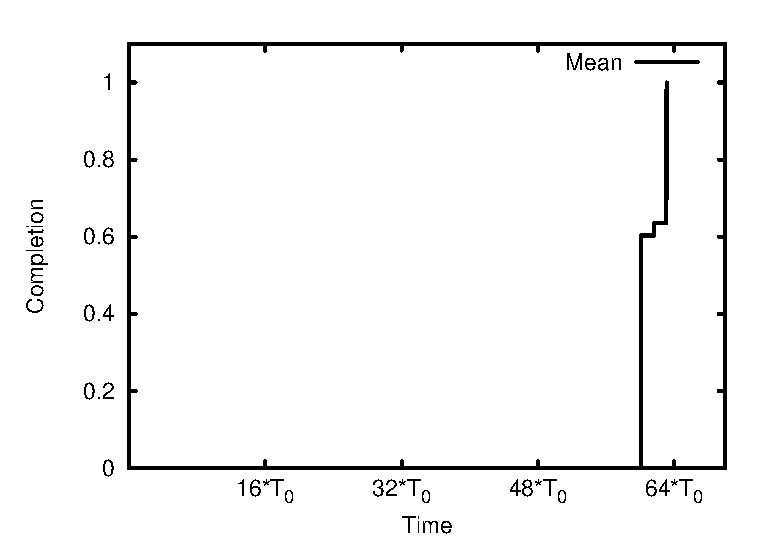
\includegraphics[width=0.5\textwidth]{plots/scenario_1_default/plots/GeneratedMeanChunkCompletion.csv}
	 	}~ % No whitespace here!
	 	\subfigure[Completion Per Peer\label{fig:s1:scompletion}]{
	 		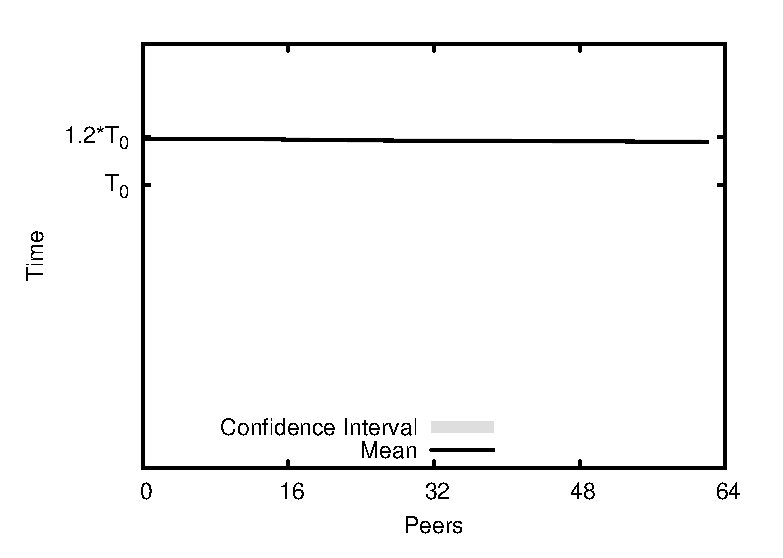
\includegraphics[width=0.5\textwidth]{plots/scenario_1_default/plots/GeneratedMeanSortedChunkCompletion.csv}
	 	}		

	 	\subfigure[Super Seeder Upload Bandwidth\label{fig:s1:ssupload}]{
	 		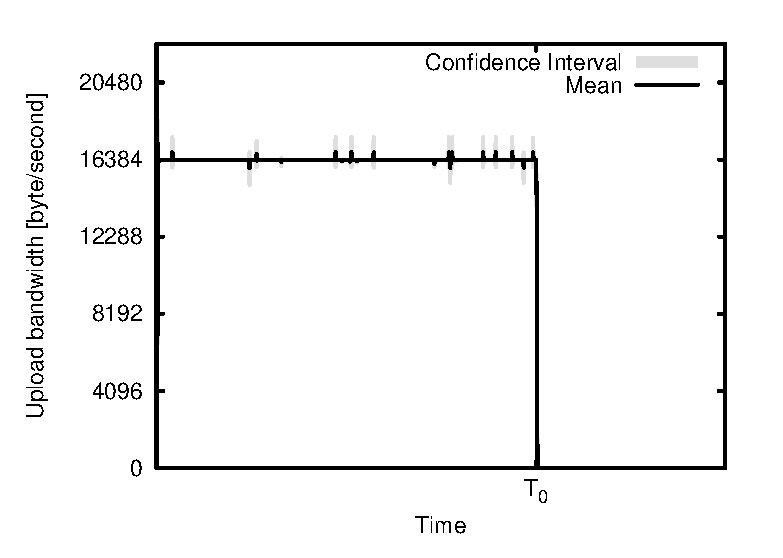
\includegraphics[width=0.5\textwidth]{plots/scenario_1_default/plots/GeneratedMeanCurrentSuperSeederUploadBandwidth.csv}
	 	}~ % No whitespace here!
	 	\subfigure[Seeder Upload Bandwidth\label{fig:s1:upload}]{
	 		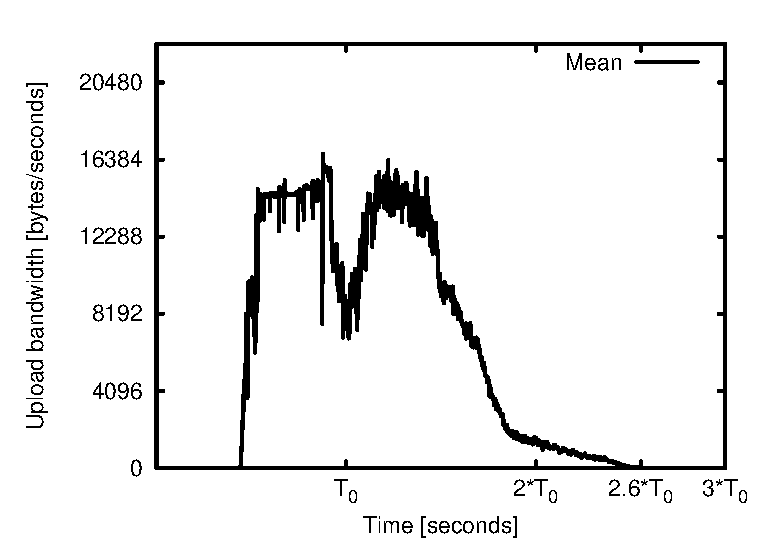
\includegraphics[width=0.5\textwidth]{plots/scenario_1_default/plots/GeneratedMeanCurrentUploadBandwidth.csv}
	 	}

	 	\subfigure[Leecher Download Bandwidth\label{fig:s1:download}]{
	 		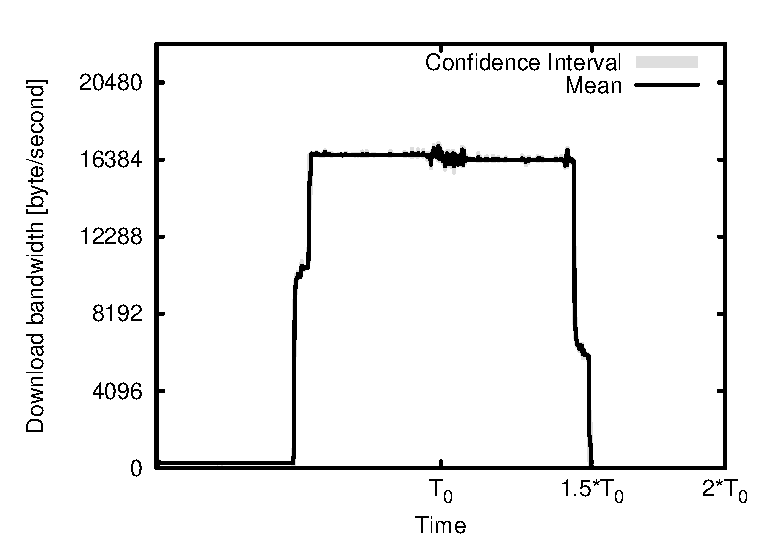
\includegraphics[width=0.5\textwidth]{plots/scenario_1_default/plots/GeneratedMeanCurrentDownloadBandwidth.csv}
	 	}
		\caption{Scenario 1 Default}
		\label{fig:s1}
	\end{center}
\end{figure}




The default scenario simulates 64 peers using the Chunked-Swarm model with super seeder extension, see Section \ref{module:algorithm:chunkedswarm}, where one peer has the complete data set at the beginning, which is called the super seeder and does only upload each chunk once. Every peer has a simulated upload bandwidth of $16.384\:\frac{bytes}{seconds}$. The download bandwidth is not limited. The size of the data set is not specified directly, but is calculated from the upload bandwidth and $T_0$, which is set to ten minutes (600 seconds). So a single transfer from the super seeder to one peer takes exactly $T_0$ seconds. The small upload bandwidth has a major advantage for benchmarking, because basically it represents the buffer size of each peer. So $n\:*\:u$ is the minimal memory usage of a benchmark, where $n$ is the number of peers and $u$ the upload bandwidth. If the upload bandwidth is too high, the overhead of the memory usage will influence the expressiveness of the benchmark. Since the size of the data set is always relative to the upload bandwidth and $T_0$, the actual upload bandwidth does not matter. The data set is also splitted into twice as many chunks as there are peers, but without the super seeder, which makes $63\:*\:2=126$ chunks. The default scenario also simulates a meta data size of one byte. In reality, the meta data would be something about 64 bytes, because it contains a \emph{SHA-1} hash, a bit set and some network protocol headers, but because the upload bandwidth is reduced for the benchmark, the meta data size should be reduced as well. In this special case the $\frac{16.384\:\frac{bytes}{seconds}}{1\:byte}$ ratio is equal to $\frac{1.048.576\:\frac{bytes}{seconds}}{64\:bytes}$. So if we assume, that a usual peer has an upload bandwidth of $1.048.576\:\frac{bytes}{second}$, which is quite common these days, the benchmark values are realistic.

Figure \ref{fig:s1:completion} shows the mean completion graph for each peer, where the x-axis represents the time and the y-axis the completion of the data set from $0.0$ to $1.0$. After $1.5\:*\:T_0$ every peer has the complete data set available. As shown in Chapter \ref{theory}, the formula $T(n, c) = (1\:+\:\frac{n-1}{c})\:T_0$ calculates the time needed for the Chunked-Swarm model. So $c\:=126$, $n\:=\:63$ and $T(63, 126) = (1\:+\:\frac{63-1}{126})\:T_0 = 1,49\:T_0$. Figure \ref{fig:s1:scompletion} shows the mean completion time of all 63 peers, sorted in descending order. Since this graph is almost a horizontal line, all peers complete the transfer roughly at the same time.

Figure \ref{fig:s1:ssupload} shows the mean super seeder upload bandwidth. For $T_0$ seconds, the super seeder uploads at full speed after which it stops uploading, because the super seeder extension forbids uploading the same chunk twice, so every chunk is uploaded once. Figure \ref{fig:s1:upload} and Figure \ref{fig:s1:download} present the mean upload and download bandwidth of all remaining peers. Since there are twice as many chunks as peers, each peer can start uploading chunks after $0.5\:*\:T_0$ seconds, as described in Section \ref{theory:model:chunkedswarm}. It is important to note that the distribution phase and the super seeder run in parallel after $0.5\:*\:T_0$ seconds.


 































